\graphicspath{ {images/} }

% real numbers R symbol
\newcommand{\Real}{\mathbb{R}}

% encoder hidden
\newcommand{\henc}{\bh^{\text{enc}}}
\newcommand{\hencfw}[1]{\overrightarrow{\henc_{#1}}}
\newcommand{\hencbw}[1]{\overleftarrow{\henc_{#1}}}

% encoder cell
\newcommand{\cenc}{\bc^{\text{enc}}}
\newcommand{\cencfw}[1]{\overrightarrow{\cenc_{#1}}}
\newcommand{\cencbw}[1]{\overleftarrow{\cenc_{#1}}}

% decoder hidden
\newcommand{\hdec}{\bh^{\text{dec}}}

% decoder cell
\newcommand{\cdec}{\bc^{\text{dec}}}

\titledquestion{Neural Machine Translation with RNNs}[45]
 In Machine Translation, our goal is to convert a sentence from the \textit{source} language (e.g. Mandarin Chinese) to the \textit{target} language (e.g. English). In this assignment, we will implement a sequence-to-sequence (Seq2Seq) network with attention, to build a Neural Machine Translation (NMT) system. In this section, we describe the \textbf{training procedure} for the proposed NMT system, which uses a Bidirectional LSTM Encoder and a Unidirectional LSTM Decoder.\newline

\begin{figure}[h]
    \begin{center}
        \captionsetup{width=0.8\textwidth}
        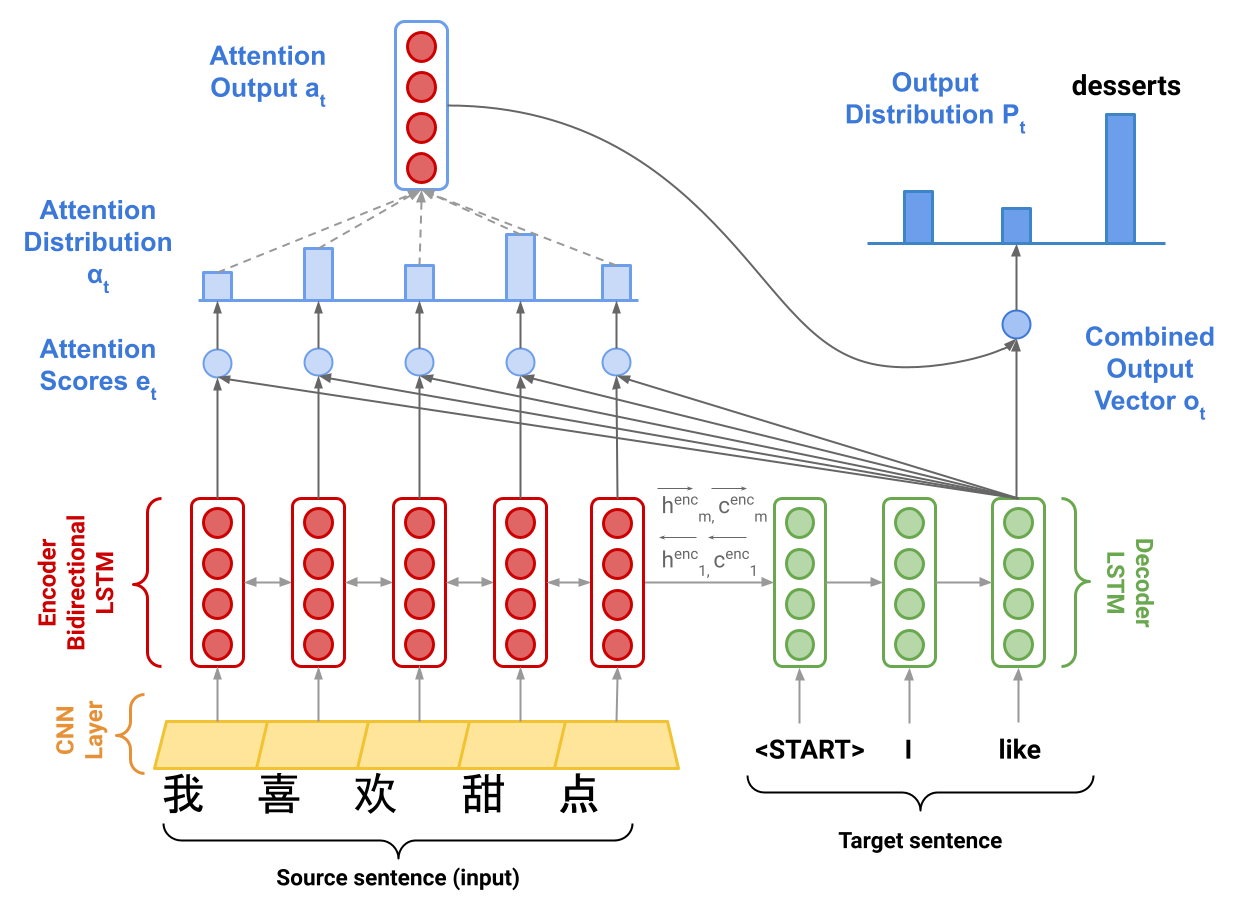
\includegraphics[width=0.8\textwidth]{images/Assignment 4 Figure.png}
        \caption{Seq2Seq Model with Multiplicative Attention, shown on the third step of the decoder. Hidden states $\henc_i$ and cell states $\cenc_i$ are defined on the next page.
        }
        \label{nmt-figure}
    \end{center}
\end{figure}

\subsection*{Model description (training procedure)}
 Given a sentence in the source language, we look up the character or word embeddings from an \textbf{embeddings matrix}, yielding $\bx_1, \dots, \bx_m$ ($\bx_i \in \Real^{e \times 1}$), where $m$ is the length of the source sentence and $e$ is the embedding size. We then feed the embeddings to a \textbf{convolutional layer} \footnote{Checkout \url{https://cs231n.github.io/convolutional-networks} for an in-depth description for convolutional layers if you are not familiar} while maintaining their shapes. We feed the convolutional layer outputs to the \textbf{bidirectional encoder}, yielding hidden states and cell states for both the forwards ($\rightarrow$) and backwards ($\leftarrow$) LSTMs. The forwards and backwards versions are concatenated to give hidden states $\henc_i$ and cell states $\cenc_i$:
 
\begin{align}
    \henc_i = [\hencbw{i}; \hencfw{i}] \enspace &\text{where}\enspace \henc_i \in \Real^{2h \times 1}, \hencbw{i}, \hencfw{i} \in \Real^{h \times 1} &1 \le i \le m \\
    \cenc_i = [\cencbw{i}; \cencfw{i}] \enspace &\text{where} \enspace \cenc_i \in \Real^{2h \times 1}, \cencbw{i}, \cencfw{i} \in \Real^{h \times 1} &1 \le i \le m
\end{align}

We then initialize the \textbf{decoder}'s first hidden state $\hdec_0$ and cell state $\cdec_0$ with a linear projection of the encoder's final hidden state and final cell state.\footnote{If it's not obvious, think about why we regard $[\hencbw{1}, \hencfw{m}]$ as the `final hidden state' of the Encoder.} 

\begin{align}
    \hdec_0 = \bW_{h}[\hencbw{1}; \hencfw{m}] \enspace &\text{where} \enspace \hdec_0 \in \Real^{h \times 1}, \bW_{h} \in \Real^{h \times 2h}\\
    \cdec_0 = \bW_{c}[\cencbw{1}; \cencfw{m}] \enspace &\text{where} \enspace \cdec_0 \in \Real^{h \times 1}, \bW_{c} \in \Real^{h \times 2h}
\end{align}

With the decoder initialized, we must now feed it a target sentence. On the $t^{th}$ step, we look up the embedding for the $t^{th}$ subword,  $\by_t \in \Real^{e \times 1}$. We then concatenate $\by_t$ with the \textit{combined-output vector} $\bo_{t-1} \in \Real^{h \times 1}$ from the previous timestep (we will explain what this is later down this page!\@) to produce $\overline{\by_t} \in \Real^{(e+h) \times 1}$. Note that for the first target subword (i.e. the start token) $\bo_{0}$ is a zero-vector. We then feed $\overline{\by_t}$ as input to the decoder. 

\begin{align}
    \hdec_t, \cdec_t = \text{Decoder}(\overline{\by_t}, \hdec_{t-1}, \cdec_{t-1}) \enspace &\text{where} \enspace \hdec_t \in \Real^{h \times 1}, \cdec_t \in \Real^{h \times 1}\\
\end{align}

We then use $\hdec_t$ to compute  multiplicative attention over $\henc_1, \dots, \henc_m$:

\begin{align}
    \be_{t, i} = (\hdec_t)^T\bW_{\text{attProj}}\henc_i \enspace &\text{where} \enspace \be_{t} \in \Real^{m \times 1}, \bW_{\text{attProj}}\in \Real^{h \times 2h} & 1 \le i \le m \\
    \alpha_t= \text{softmax}(\be_t) \enspace &\text{where} \enspace \alpha_t \in \Real^{m \times 1}\\
    \ba_t = \sum_{i=1}^{m}\alpha_{t,i}\henc_i \enspace &\text{where} \enspace \ba_t \in \Real^{2h \times 1}
\end{align}
 
$\be_{t, i}$ is a scalar, the $i$th element of $\be_{t} \in \Real^{m \times 1}$, computed using the hidden state of the decoder at the $t$th step, $\hdec_t \in \Real^{h \times 1}$, the attention projection $\bW_{\text{attProj}} \in \Real^{h \times 2h}$, and the hidden state of the encoder at the $i$th step, $\henc_i \in \Real^{2h \times 1}$.

We now concatenate the attention output $\ba_t$ with the decoder hidden state $\hdec_t$ and pass this through a linear layer, tanh, and dropout to attain the \textit{combined-output} vector $\bo_{t}$.

\begin{align}   
    \bu_{t} = [\ba_{t}; \hdec_t] \enspace &\text{where} \enspace \bu_t \in  \Real^{3h \times 1} \\
    \bv_t = \bW_{u}\bu_t \enspace &\text{where} \enspace \bv_t \in \Real^{h \times 1}, \bW_{u} \in \Real^{h \times 3h}\\
    \bo_t = \text{dropout}(\text{tanh}(\bv_t)) \enspace &\text{where} \enspace \bo_t \in \Real^{h \times 1}
\end{align}

Then, we produce a probability distribution $\bP_t$ over target subwords at the $t^{th}$ timestep:

\begin{align}
    \bP_t = \text{softmax}(\bW_{\text{vocab}}\bo_{t}) \enspace &\text{where} \enspace \bP_t \in \Real^{V_{t} \times 1}, \bW_{\text{vocab}} \in \Real^{V_{t} \times h}
\end{align}

Here, $V_{t}$ is the size of the target vocabulary. Finally, to train the network we then compute the cross entropy loss between $\bP_t$ and $\bg_{t}$, where $\bg_{t}$ is the one-hot vector of the target subword at timestep $t$:

\begin{align}
    J_t(\theta) = \mathrm{CrossEntropy}(\bP_t,\bg_{t})
\end{align}

Here, $\theta$ represents all the parameters of the model and $J_t(\theta)$ is the loss on step $t$ of the decoder.
Now that we have described the model, let's try implementing it for Mandarin Chinese to English translation!

\subsection*{Setting up your Virtual Machine}
Follow the instructions in the \href{https://docs.google.com/document/d/11kRyfClhTi4-MC1feWWCMI31fHpTzddASsDa48_Dd9E/edit?usp=sharing}{CS224n Azure Guide} (link also provided on website and Ed) in order to create your VM instance. This should take you approximately 45 minutes. Though you will need the GPU to train your model, we strongly advise that you first develop the code locally and ensure that it runs, before attempting to train it on your VM. GPU time is expensive and limited. It takes approximately \textbf{1.5 to 2 hours} to train the NMT system. We don't want you to accidentally use all your GPU time for debugging your model rather than training and evaluating it. Finally, \textbf{make sure that your VM is turned off whenever you are not using it.}

\textbf{\textcolor{red}{If your Azure subscription runs out of money, your VM will be temporarily locked and inaccessible. If that happens, please fill out a request form \href{https://forms.gle/PUwiA1rR5aQNWxYt6}{here}.}}

In order to run the model code on your \textbf{local} machine, please run the following command to create the proper virtual environment:

\begin{lstlisting}
    conda env create --file local_env.yml
\end{lstlisting}

Note that this virtual environment \textbf{will not} be needed on the VM.\newline

\subsection*{Implementation and written questions}

\begin{parts}
    \part [2] (coding) In order to apply tensor operations, we must ensure that the sentences in a given batch are of the same length. Thus, we must identify the longest sentence in a batch and pad others to be the same length. Implement the \texttt{pad\_sents} function in \texttt{utils.py}, which shall produce these padded sentences.
    
    \part[3] (coding) Implement the \texttt{\_\_init\_\_} function in \texttt{model\_embeddings.py} to initialize the necessary source and target embeddings.

    \part[4] (coding) Implement the \texttt{\_\_init\_\_} function in \texttt{nmt\_model.py} to initialize the necessary model layers (LSTM, CNN, projection, and dropout) for the NMT system.
    
    \part[8] (coding) Implement the \texttt{encode} function in \texttt{nmt\_model.py}. This function converts the padded source sentences into the tensor $\bX$, generates $\henc_1, \dots, \henc_m$, and computes the initial state $\hdec_0$ and initial cell $\cdec_0$ for the Decoder. You can run a non-comprehensive sanity check by executing:
    
\begin{lstlisting}
    python sanity_check.py 1d
\end{lstlisting}
    
    \part[8] (coding) Implement the \texttt{decode} function in \texttt{nmt\_model.py}. This function constructs $\bar{\by}$ and runs the \texttt{step} function over every timestep for the input. You can run a non-comprehensive sanity check by executing:

     
\begin{lstlisting}
    python sanity_check.py 1e
\end{lstlisting}
    
    \part[10] (coding) Implement the \texttt{step} function in \texttt{nmt\_model.py}. This function applies the Decoder's LSTM cell for a single timestep, computing the encoding of the target subword $\hdec_t$, the attention scores $\be_t$, attention distribution $\alpha_t$, the attention output $\ba_{t}$, and finally the combined output $\bo_t$. You can run a non-comprehensive sanity check by executing:
    
    
\begin{lstlisting}
    python sanity_check.py 1f
\end{lstlisting}
           
    
    \part [3] (written) The \texttt{generate\_sent\_masks()} function in \texttt{nmt\_model.py} produces a tensor called \texttt{enc\_masks}. It has shape (batch size, max source sentence length) and contains 1s in positions corresponding to `pad' tokens in the input, and 0s for non-pad tokens. Look at how the masks are used during the attention computation in the \texttt{step()} function (lines 311-312). 
    
    First explain (in around three sentences) what effect the masks have on the entire attention computation.
    Then explain (in one or two sentences) why it is necessary to use the masks in this way.

    \ifans{}
\end{parts}

Now it's time to get things running! As noted earlier, we recommend that you develop the code on your personal computer.  Confirm that you are running in the proper conda environment and then execute the following command to train the model on your local machine:
    
\begin{lstlisting}
    sh run.sh train_local
    (Windows) run.bat train_local
\end{lstlisting}

For a faster way to debug by training on less data, you can run the following instead:
\begin{lstlisting}
    sh run.sh train_debug
    (Windows) run.bat debug
\end{lstlisting}


To help with monitoring and debugging, the starter code uses tensorboard to log loss and perplexity during training using TensorBoard\footnote{https://pytorch.org/docs/stable/tensorboard.html}. TensorBoard provides tools for logging and visualizing training information from experiments. To open TensorBoard, run the following in your conda environment:

\begin{lstlisting}
   tensorboard --logdir=runs
\end{lstlisting}

You should see a significant decrease in loss during the initial iterations. Once you have ensured that your code does not crash (i.e. let it run till \texttt{iter 10} or \texttt{iter 20}), power on your VM from the Azure Web Portal. Then read the \textit{Managing Code Deployment to a VM} section of our \href{https://docs.google.com/document/d/11kRyfClhTi4-MC1feWWCMI31fHpTzddASsDa48_Dd9E/edit?usp=sharing}{Practical Guide to VMs} (link also given on website and Ed) for instructions on how to upload your code to the VM.

Next, install necessary packages to your VM by running:
    
\begin{lstlisting}
    pip install -r gpu_requirements.txt
\end{lstlisting}

Finally, turn to the \textit{Managing Processes on a VM} section of the Practical Guide and follow the instructions to create a new tmux session. Concretely, run the following command to create tmux session called \texttt{nmt}. 
\begin{lstlisting}
    tmux new -s nmt
\end{lstlisting}


Once your VM is configured and you are in a tmux session, execute:
\begin{lstlisting}
    sh run.sh train
    (Windows) run.bat train
\end{lstlisting}
    
Once you know your code is running properly, you can detach from session and close your ssh connection to the server. To detach from the session, run:
\begin{lstlisting}
    tmux detach
\end{lstlisting}
    
You can return to your training model by ssh-ing back into the server and attaching to the tmux session by running:
    
\begin{lstlisting}
    tmux a -t nmt
\end{lstlisting}

\begin{parts}
\setcounter{partno}{7}
\part[3] (written) Once your model is done training (\textbf{this should take under 2 hours on the VM}), execute the following command to test the model:
\begin{lstlisting}
sh run.sh test
(Windows) run.bat test
\end{lstlisting}
    Please report the model's corpus BLEU Score. It should be larger than 18.
    
    \ifans{}
    
    \part[4] (written) In class, we learned about dot product attention, multiplicative attention, and additive attention.  As a reminder, dot product attention is $\be_{t,i} = \bs_t^T\bh_i$, multiplicative attention is $\be_{t,i} = \bs_t^T\bW\bh_i$, and additive attention is $\be_{t,i} = \bv^T \text{tanh}(\bW_1\bh_i + \bW_2\bs_t)$.
    
    \begin{subparts}
    \subpart[2] Explain one advantage and one disadvantage of \textit{dot product attention} compared to multiplicative attention.
    \subpart[2] Explain one advantage and one disadvantage of \textit{additive attention} compared to multiplicative attention.
    \end{subparts}
            
    \ifans{}
\end{parts}
